\section{Introduction} \label{sec:intro}

The main motivation for graph drawing and geometric representations is finding ways
to visualize some given data efficiently. The most famous representations are plane drawings, in
which we draw a graph in the plane and we want to avoid (or minimize) crossings of edges.
However, for certain types of graphs, \emph{intersection representations} are more suitable.  They
represent each vertex by a geometrical object and encode the edges by intersections.

\subsection{Interval Graphs}

The most studied class of intersection graphs are \emph{interval graphs} (\int), defined by
H\'ajos~\cite{hajos_interval_graphs} in 1957. An \emph{interval representation} $\calR$ is a
collection of closed intervals $\bigl\{\inter x : x \in V(G)\bigr\}$ where $\inter x \cap \inter y
\ne \emptyset$ if and only if $xy \in E(G)$. A graph is an interval graph if it has an interval
representation; see Fig.~\ref{fig:int_example}a.

\begin{figure}[b!]
\centering
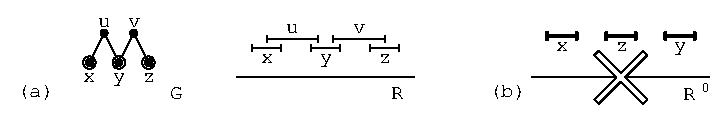
\includegraphics{introduction_int_example.eps}
\caption{(a) An interval graph $G$ with one of its interval representations $\calR$.  (b) A partial
representation $\calR'$ with pre-drawn intervals $\inter x'$, $\inter y'$ and $\inter z'$. It is
non-extendible since $\inter u$ cannot be placed. In all figures, we depict pre-drawn intervals in
bold.}
\label{fig:int_example}
\end{figure}

Interval graphs have many applications. Already in 1959, Benzer~\cite{benzer_interval_graphs} used
them in his experimental study of DNA. For some time, interval graphs played an important role for
the DNA hybridization~\cite{karp_hybridization}, in which short pieces of DNA are studied
independently. Further applications include scheduling, psychology, archaeology,
etc.~\cite{stoffers,roberts_discrete_models,kendall}.

Interval graphs also have nice theoretical properties. They are perfect and closely related to
path-width decompositions. They can be recognized in linear
time~\cite{PQ_trees,LBFS_int,finding_lb_graphs}, and many hard combinatorial problems are
polynomially solvable for interval graphs.  Fulkerson and Gross~\cite{maximal_cliques} characterized
them by consecutive orderings of maximal cliques (see Section~\ref{sec:maximal_cliques} for
details).  This lead Booth and Lueker~\cite{PQ_trees} to the construction of PQ-trees, which are an
efficient data structure to deal with consecutive orderings, and have many other applications. 

\emph{Chordal graphs} (\chor) are graphs with no induced cycle of length four or more, alternatively
intersection graphs of subtrees of trees. Three vertices form an \emph{asteroidal triple} if there
exists a path between every pair of them avoiding the neighborhood of the third vertex.
\emph{Asteroidal triple-free graphs} (\atfree) are graphs containing no asteroidal triples.
Lekkerkerker and Boland~\cite{lb_graphs} characterized interval graphs as $\int = \chor \cap
\atfree$. They described this characterization by the minimal forbidden induced subgraphs given in
Fig.~\ref{fig:LB_obstructions} which we call \emph{Lekkerkerker-Boland obstructions} (LB).

\begin{figure}[t!]
\centering
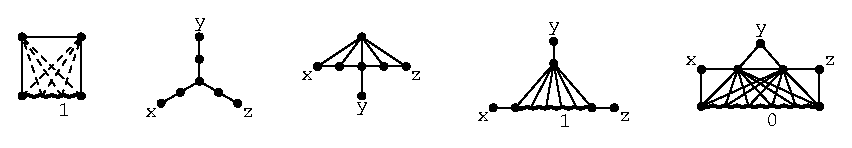
\includegraphics{introduction_LB_obstructions.eps}
\caption{Five types of LB obstructions which are the minimal forbidden induced subgraphs of \int.
The bold curly lines correspond to induced paths with denoted minimal lengths. The leftmost
obstructions are induced cycles of length four or more.  The remaining four types of obstructions
are minimal asteroidal triples $(x,y,z)$ which are chordal graphs.}
\label{fig:LB_obstructions}
\end{figure}

\subsection{Partial Representation Extension}

The partial representation extension problem was introduced by Klav\'{\i}k et al.~\cite{kkv}.  A
\emph{partial representation} $\calR'$ of $G$ is an interval representation $\bigl\{\inter x' : x \in
V(G')\bigr\}$ of an induced subgraph $G'$ of $G$. The vertices of $G'$ and the intervals of $\calR'$
are called \emph{pre-drawn}.  A representation $\calR$ of $G$ \emph{extends} $\calR'$ if and only if
it assigns the same intervals to the vertices of $G'$, i.e., $\inter x = \inter x'$ for every $x \in
V(G')$.  For an example, see Fig.~\ref{fig:int_example}b.

\computationproblem
{Partial Representation Extension -- $\ext(\int)$}
{A graph $G$ and a partial representation $\calR'$ of $G'$.}
{Is there an interval representation of $G$ extending $\calR'$?}
{9.25cm}

\noindent The first polynomial-time algorithm, running in $\O(n^2)$ time, was given in~\cite{kkv}.
Currently, there are two different linear-time algorithms~\cite{blas_rutter,kkosv} for this problem.
	
We note that the partial representation extension problems have been considered also for other classes
of intersection graphs. A linear-time algorithm for proper interval graphs and an almost quadratic-time
algorithm for unit interval graphs are given in~\cite{kkorssv}, and improved to quadratic time
in~\cite{soulignac}. The partial representation extension problems are polynomial-time solvable for
$k$-nested interval graphs (classes generalizing proper interval graphs), but \cNP-hard for
$k$-length interval graphs (classes generalizing unit interval graphs), even for $k=2$~\cite{kos}.
Polynomial-time algorithms are further known for circle graphs~\cite{cfk}, and
permutation and function graphs~\cite{kkkw}. The partial representation extension problems for
chordal graphs~\cite{kkos} and contact representations of planar graphs~\cite{contact_planar_ext}
are \cNP-hard. Notable graph classes for which the complexity of the partial representation
extension problem is open are circular-arc graphs and trapezoid graphs.

Outside intersection graphs, the similar problem was considered even sooner for planar
graphs.  Partially embedded planar graphs can be extended in linear time~\cite{extending_planar}.
Even though every planar graph has a straight-line embedding, extension of such embeddings is
\cNP-hard~\cite{straight_planar_npcomplete}. Kuratowski's characterization of minimal forbidden
minors was extended to partially embedded planar graphs by Jel\'{\i}nek et
al.~\cite{kuratowski_ext}. Our research has a similar spirit as this last result.

\begin{figure}[b!]
\centering
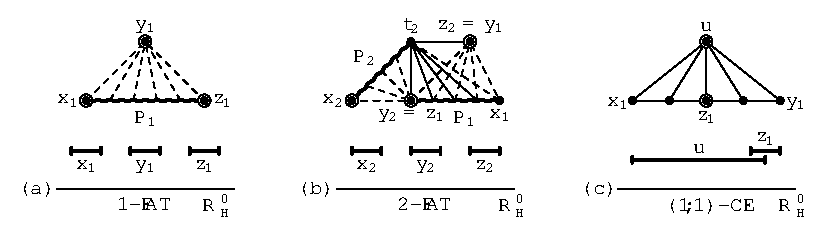
\includegraphics{introduction_minimal_obstructions.eps}
\caption{Three examples of minimal obstructions, each consisting of a graph $H$ and a non-extendible
partial representation $\calR'_H$. Curly lines denote induced paths and dashed edges are non-edges.
The obstructions (a) and (b) are the first two $k$-FAT obstructions, and (c) is the simplest
$(k,\ell)$-CE obstruction.}
\label{fig:minimal_obstructions}
\end{figure}

\subsection{Our Results}

In this paper, we generalize the characterization of Lekkerkerker and Boland~\cite{lb_graphs} to
describe minimal obstruction which make partial representations non-extendible.  Each obstruction
consists of a small graph and its non-extendible partial representation.  Aside LB obstructions, we have
two trivial obstructions, called SE, and ten infinite classes of minimal obstructions. The main
class, called $k$-FAT obstructions, has three wrongly ordered disjoint pre-drawn intervals
$\inter{x_k}'$, $\inter{y_k}'$, and $\inter{z_k}'$. The obstruction consists of a zig-zag structure
with $k$ levels where the last level cannot be placed.  See Fig.~\ref{fig:minimal_obstructions}a and
b for $1$-FAT and $2$-FAT obstructions. There are eight other infinite classes derived from $k$-FAT
obstructions by adding a few vertices and having different vertices pre-drawn. The last infinite
class of $(k,\ell)$-CE obstructions consists of a $k$-FAT obstruction glued with an $\ell$-FAT
obstruction and contains only two pre-drawn vertices; see Fig.~\ref{fig:minimal_obstructions}c for a
$(1,1)$-CE obstruction.  We formally define these minimal obstructions in
Section~\ref{sec:definition_of_obstructions}.

\begin{theorem} \label{thm:repext_obstructions}
A partial representation $\calR'$ of $G$ is extendible if and only if $G$ and $\calR'$ contain no
LB, SE, $k$-FAT, $k$-BI, $k$-FS, $k$-EFS, $k$-FB, $k$-EFB, $k$-FDS, $k$-EFDS, $k$-FNS and
$(k,\ell)$-CE obstructions.
\end{theorem}

Since every minimal obstruction contains at most four pre-drawn intervals, we get the following
Helly-type result as a straightforward corollary:

\begin{corollary} \label{cor:helly_obstructions}
A partial representation is extendible if and only if every quadruple of pre-drawn intervals is
extendible by itself.
\end{corollary}

All known algorithms for the partial representation extension problems
\cite{kkv,kkkw,blas_rutter,kkosv,kkorssv,kkos} are able to certify solvable instances by outputting
an extending representation. Using our minimal obstructions, we construct the first algorithm for
partial representation extension certifying also non-extendible partial
representations.\footnote{Formally speaking, a polynomial-time algorithm certifies
unsolvable instances by outputting ``no'' and by a proof of its correctness. Our algorithm
outputs a simple proof that a given partial representation is non-extendible in terms of a
minimal obstruction. This proof can be independently verified which is desirable.}

\begin{corollary} \label{cor:certifying_algorithm}
Assume that the input gives the endpoints in a partial representation sorted from left to right.
Then there exists an $\O(n+m)$ certifying algorithm for the partial representation extension problem,
where $n$ is the number of vertices and $m$ is the number of edges of the input graph. If the answer
is ``yes'', it outputs an extending representation. If the answer is ``no'', it detects one of the
minimal obstructions.
\end{corollary}

\heading{Outline.} In Section~\ref{sec:definition_of_obstructions}, we define the minimal
obstructions which make a partial representation non-extendible. In
Section~\ref{sec:maximal_cliques}, we introduce the standard tools for working with interval graphs:
the characterization of Fulkerson and Gross by linear orderings of maximal cliques, and the related
data structure called an MPQ-trees which stores all feasible orderings.

In Section~\ref{sec:interval_orders}, we restate the characterization of~\cite{kkosv}: a partial
representation is extendible if and only if there exists a feasible ordering of the maximal cliques
which extends a certain partial ordering $\wlt$. Therefore, to solve $\ext(\int)$, we test whether
the MPQ-tree can be reordered according $\wlt$.

Based on this, in Section~\ref{sec:strategy}, we build our strategy for showing that every
non-extendible partial representation contains one of the defined minimal obstructions. If
reordering of the MPQ-tree according to $\wlt$ fails, then it fails in a leaf, in a P-node, or a
Q-node. We deal with these three cases in Sections~\ref{sec:leaves}, \ref{sec:p_nodes},
and~\ref{sec:q_nodes}, respectively, where the last one is most involved. In
Section~\ref{sec:main_result}, we put these results together and establish
Theorem~\ref{thm:repext_obstructions} and Corollaries~\ref{cor:helly_obstructions}
and~\ref{cor:certifying_algorithm}.

We conclude with a discussion of our results and several open problems.

\subsection{Preliminaries}

For a graph $G$, we denote by $V(G)$ its vertices and by $E(G)$ its edges. We denote the
\emph{closed neighborhood} of $x$ by $N[x]$. Maximal cliques are denoted by the letters $a$ to $f$,
and vertices by the remaining letters. For $A \subseteq V(G)$, we denote by $G[A]$ the subgraph
induced by $A$. Similarly, for $A \subseteq V(G')$, we denote by $\calR'[A]$ the partial
representations which only contains the pre-drawn intervals in $A$. By $P_{x,y}$ we denote an
induced path from $x$ to $y$; its length is the number of edges.

For an interval $\inter x$, we denote its left endpoint by $\ell(x)$ and its right endpoint by
$r(x)$. If $r(x) < \ell(y)$, we say that $\inter x$ is \emph{on the left} of $\inter y$ and $\inter
y$ is \emph{on the right} of $\inter x$. We say that $\inter y$ is \emph{between} $\inter x$ and
$\inter z$ if $\inter x$ is on the left of $\inter y$ and $\inter z$ is on the right of $\inter y$,
or vice versa. We also work with open intervals, for which the inequalities are non-strict.

We conclude with a list of the remaining notation.  In Section~\ref{sec:maximal_cliques}, we define
MPQ-trees, $s(N)$, $s_i(Q)$, $s^{\lft}_u(Q)$, $s^{\rt}_u(Q)$, $G[T]$, $G[N]$, $T[N]$, and
$Q$-monotone paths. In Section~\ref{sec:interval_orders}, we define $\clql(a)$, $\clqr(a)$, $I_a$,
$\wlt$, the flip operation, $P^{\startrt}(a)$, and $P^{\endlft}(a)$.
